\documentclass{beamer}
\usepackage[utf8]{inputenc}
\usepackage{tikz}
\usepackage{hyperref}

% Define colours for hyperlinks
\hypersetup{
    colorlinks=true,
    linkcolor=blue,
    filecolor=magenta,
    urlcolor=cyan,
    pdftitle={Ontology-Enhanced LLMs Presentation},
    pdfpagemode=FullScreen
}

\usetheme{Madrid}
\usecolortheme{default}

%------------------------------------------------------------
%This block of code defines the information to appear in the
%Title page
\title[Ontology-Enhanced LLMs] %optional
{Ontology-Enhanced Contextual Reasoning for Large Language Models in STEM Education}

\subtitle{Bachelor Thesis Presentation}

\author[Kinlo] % (optional)
{Kinlo Ephriam Tangiri}

\institute[Constructor University] % (optional)
{
  Department of Computer Science\\
  Constructor University\\
  \smallskip
  \small{Supervisor: Prof. Dr. Fatahi Valilai, Omid}
}

\date[May 2025] % (optional)

\logo{
\includegraphics[height=0.6cm]{bsc-logo}}

%End of title page configuration block
%------------------------------------------------------------

%------------------------------------------------------------
% Modified TOC approach - no TOC at every section
% Uncomment this if you want TOC at beginning of each section

% \AtBeginSection[]
% {
%   \begin{frame}
%     \frametitle{Table of Contents}
%     \tableofcontents[currentsection]
%   \end{frame}
% }
%------------------------------------------------------------

\begin{document}

%The next statement creates the title page.
\frame{\titlepage}

%---------------------------------------------------------
%This block of code is for the table of contents after
%the title page
\begin{frame}
\frametitle{Table of Contents}
\tableofcontents
\end{frame}
%---------------------------------------------------------

\section{Research Problem}

%---------------------------------------------------------
% Slide highlighting the research problem
\begin{frame}
\frametitle{Research Problem: LLM Hallucinations in STEM Education}

\begin{block}{The Challenge}
Large Language Models (LLMs) hallucinate a lot by generating confidently plausible but factually incorrect information.
\end{block}

\begin{itemize}
    \item<1-> LLM hallucinations occur in most technical STEM concepts
    \item<2-> In STEM education, accuracy is crucial for effective learning
    \item<3-> Traditional approaches face limitations:
    \begin{itemize}
        \item<3-> Pure LLM-based systems risk generating misinformation
        \item<3-> Rule-based systems lack natural interaction capabilities of LLMs
        \item<3-> Prompt engineering is complex and requires domain Knowledge
        \item<3-> Fine-tuning LLMs is resource-intensive, time-consuming, and requires domain Knowledge
    \end{itemize}
\end{itemize}
\end{frame}

%---------------------------------------------------------
% Slide for Research Question and Objectives
\begin{frame}
\frametitle{Research Question \& Objectives}

\begin{alertblock}{Research Question}
How can we make use of LLMs' natural language processing capabilities to enhance STEM education while ensuring their responses remain accurate and reliable?
\end{alertblock}

\begin{block}{Research Objectives}
\begin{itemize}
    \item How can we integrate domain-specific knowledge with LLM reasoning?
    \item How can we enhance contextual understanding through structured knowledge?
    \item How can we create an adaptive, personalized learning system? (Future Work)
\end{itemize}
\end{block}
\end{frame}
%---------------------------------------------------------

%---------------------------------------------------------
% Slide about ontologies and their role in knowledge representation
\begin{frame}
\frametitle{Background: Ontologies in Knowledge Representation}

\begin{block}{What are Ontologies?}
Structured frameworks that represent knowledge within specific domains, defining concepts, properties, and relationships in a machine-readable format.
\end{block}

\begin{columns}
\column{0.5\textwidth}
\textbf{Key Components}
\begin{itemize}
    \item Classes (concepts)
    \item Properties (relationships)
    \item Instances (individuals)
    \item Axioms (rules/constraints)
    \item Reasoners (inference engines)
\end{itemize}

\column{0.5\textwidth}
\textbf{Benefits for STEM Education}
\begin{itemize}
    \item \alert{Fact verification}
    \item Explicit knowledge representation
    \item Domain-specific constraints
\end{itemize}
\end{columns}
\end{frame}
%---------------------------------------------------------

\section{Methodology}

%---------------------------------------------------------
% Slide on research methodology
\begin{frame}
\frametitle{Methodology Overview}

\begin{block}{Research Approach}
Phased development approach to create an ontology-enhanced LLM system for STEM education
\end{block}

\begin{itemize}
    \item \textbf{Core Functionality}
    \begin{itemize}
        \item Environment setup and API authentication
        \item System prompt structure
    \end{itemize}
    
    \item \textbf{Knowledge Representation}
    \begin{itemize}
        \item Physics ontology development (OWL/RDF)
        \item Concept relationships and prerequisites structure
        \item Context retrieval system implementation
        \item Knowledge base integration
    \end{itemize}
\end{itemize}
\end{frame}

\section{Implementation}

%---------------------------------------------------------
% Slide on system architecture
\begin{frame}
\frametitle{System Architecture}

\begin{block}{Integrated System Components}
Our ontology-enhanced LLM system combines structured knowledge with adaptive learning capabilities
\end{block}

% System architecture diagram removed to resolve compilation issues

\begin{columns}
\column{0.48\textwidth}
\textbf{Technical Stack}
\begin{itemize}
    \item Quart web framework (async)
    \item Claude LLM API integration
    \item OWL/RDF ontology framework
\end{itemize}

\column{0.48\textwidth}
\textbf{Information Flow}
\begin{itemize}
    \item Bidirectional LLM-ontology integration
    \item Real-time fact verification
    \item Student model adaptation
\end{itemize}
\end{columns}
\end{frame}

%---------------------------------------------------------
% Slide on ontology design
\begin{frame}
\frametitle{Ontology Design for Physics Education}

\begin{alertblock}{Hierarchical Knowledge Structure}
Physics concepts organized in a machine-readable format with explicit relationships
\end{alertblock}

\begin{itemize}
    \item<1-> \textbf{Core Physics Concepts:} Force, motion, energy, momentum, waves
    \item<2-> \textbf{Relationships:} Prerequisites, dependencies, applications
    \item<3-> \textbf{Properties:} Mathematical formulas, units, constraints
    \item<4-> \textbf{Educational Metadata:} Difficulty levels, learning objectives
    \item<5-> \textbf{Integration:} OWL/RDF technologies with SPARQL queries
\end{itemize}
\end{frame}

%---------------------------------------------------------
% Slide on LLM-Ontology integration
\begin{frame}
\frametitle{LLM-Ontology Integration}

\begin{figure}
\centering
\begin{tabular}{ccc}
\fbox{\begin{minipage}{2.5cm}\centering\textbf{LLM}\end{minipage}} & 
$\xrightarrow{\text{queries}}$ & 
\fbox{\begin{minipage}{2.5cm}\centering\textbf{Ontology}\end{minipage}} \\
 & $\xleftarrow{\text{validates}}$ & 
\end{tabular}
\end{figure}

\begin{columns}
\column{0.5\textwidth}
\textbf{Integration Mechanisms}
\begin{itemize}
    \item SPARQL query generation
    \item Dynamic context augmentation
    \item Fact verification pipeline
\end{itemize}

\column{0.5\textwidth}
\textbf{Prompt Engineering}
\begin{itemize}
    \item Ontology-aware prompts
    \item Chain-of-thought reasoning
    \item Self-verification steps
\end{itemize}
\end{columns}
\end{frame}

\section{Evaluation}

%---------------------------------------------------------
% Slide on evaluation methodology
\begin{frame}
\frametitle{Evaluation Methodology}

\begin{alertblock}{Evaluation Framework}
Modular implementation with statistical analysis and visualization components
\end{alertblock}

\begin{columns}
\column{0.5\textwidth}
\textbf{Testing Approach}
\begin{itemize}
    \item Force Concept Inventory (FCI) dataset
    \item Baseline vs. ontology-enhanced model
    \item Multiple-choice + explanation prompts
    \item Hybrid hallucination detection:
    \begin{itemize}
        \item Keyword matching
        \item Expert verification
    \end{itemize}
\end{itemize}

\column{0.5\textwidth}
\textbf{Evaluation Metrics}
\begin{itemize}
    \item Hallucination rate
    \item Trade-off analysis
\end{itemize}
\end{columns}
\end{frame}

%---------------------------------------------------------
% Slide on evaluation results
\begin{frame}
\frametitle{Results: Quantitative Analysis}

\begin{columns}
\column{0.5\textwidth}
\begin{center}
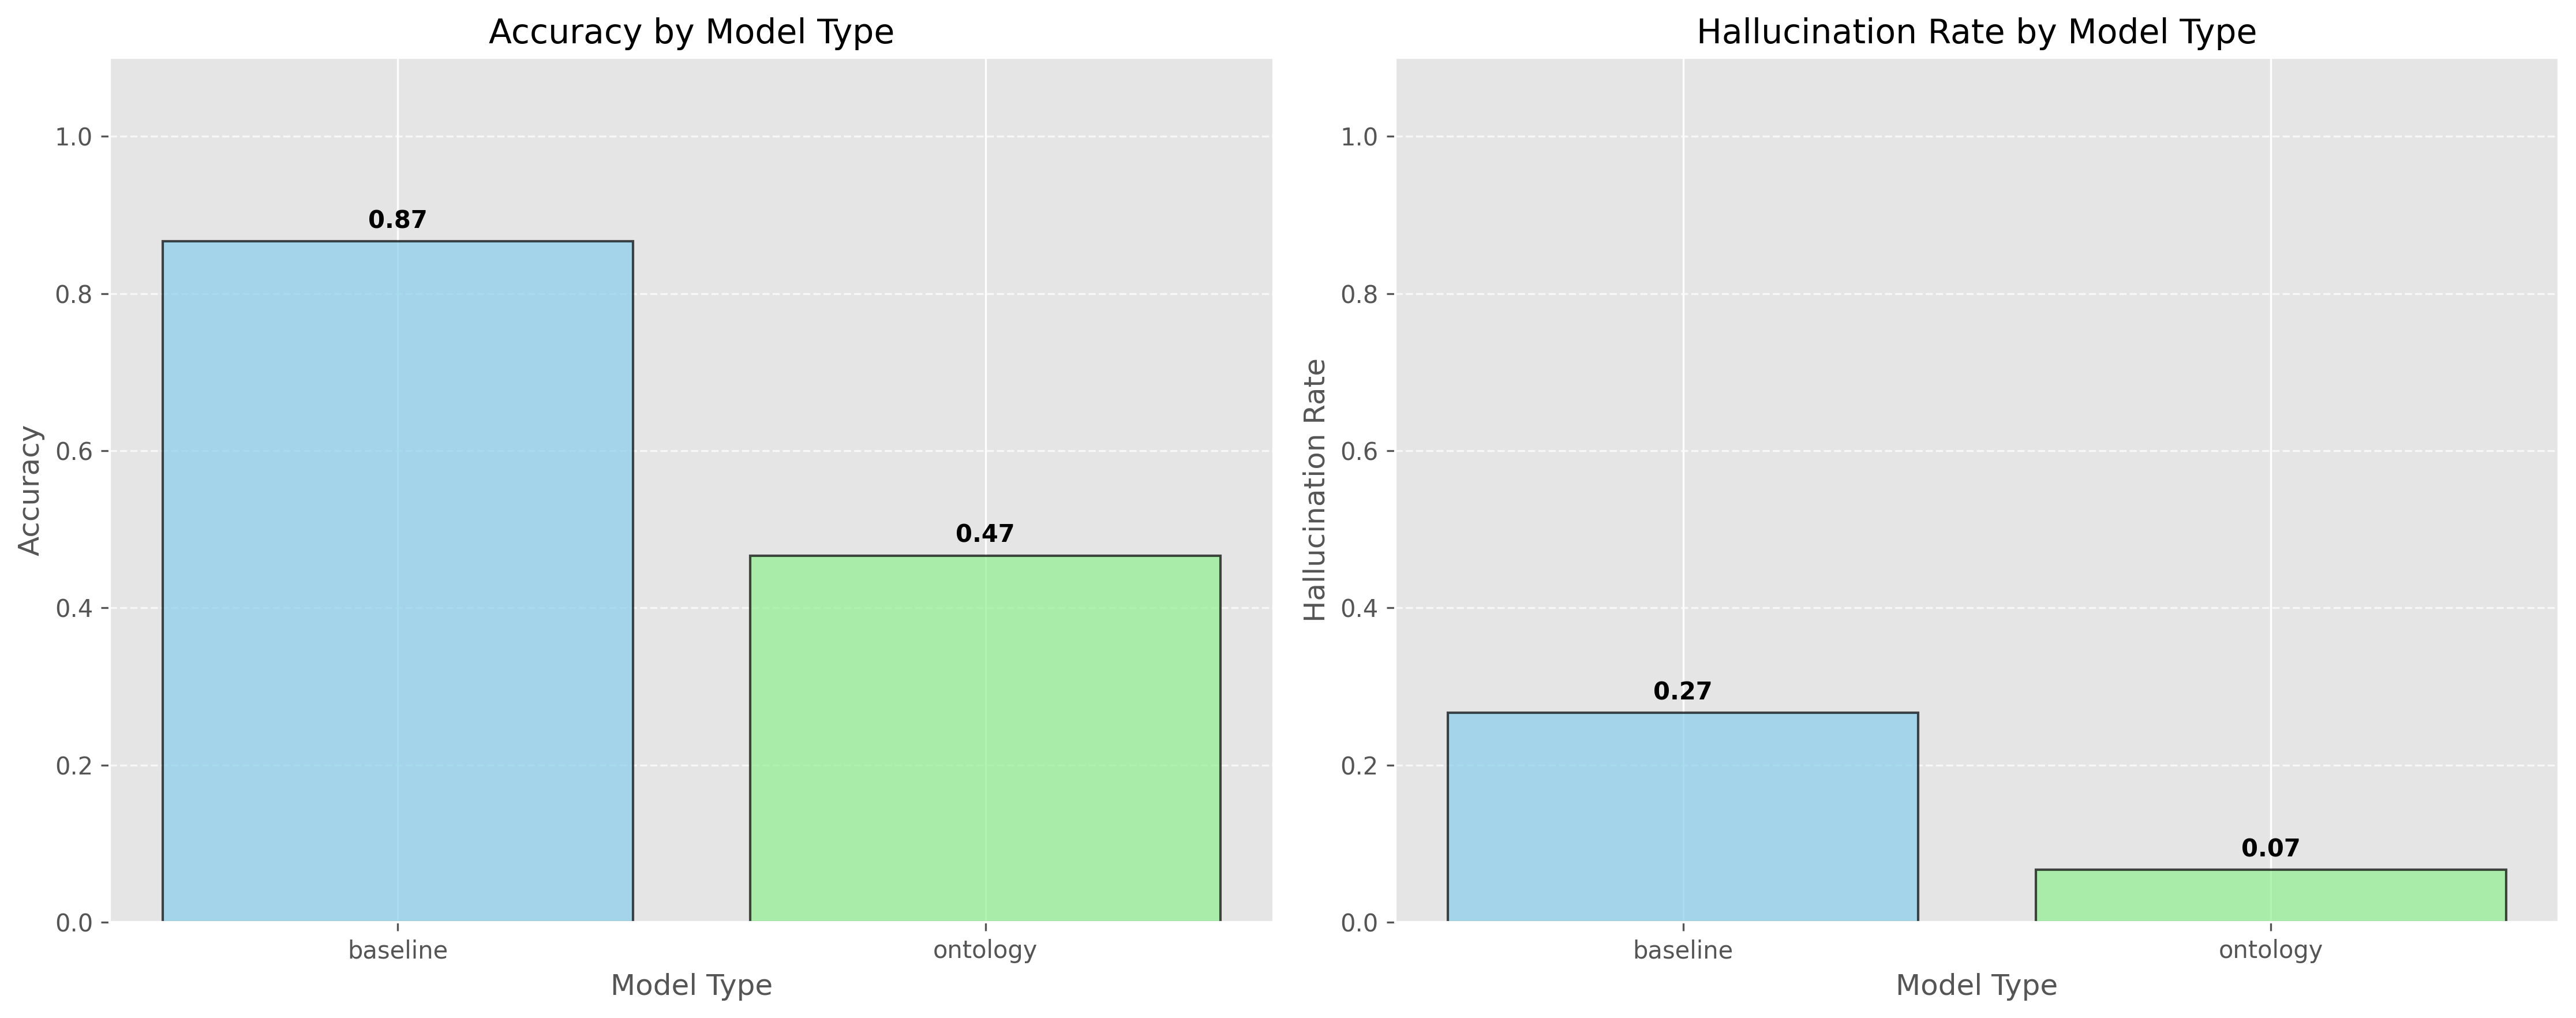
\includegraphics[width=\textwidth]{../results_final/model_comparison.png}
\end{center}

\column{0.5\textwidth}
\begin{alertblock}{Hallucination Reduction}  
\textbf{75\%} reduction (26.67\% → 6.67\%)
\end{alertblock}

\begin{itemize}
    \item \alert{Key trade-off}: Accuracy decreased from 86.67\% to 46.67\%
    \item Better for explanations than assessment
\end{itemize}
\end{columns}
\end{frame}

%---------------------------------------------------------
% Slide on educational impact
\begin{frame}
\frametitle{Educational Impact Analysis}

\begin{columns}
\column{0.5\textwidth}
\begin{block}{Case Study: Free Fall Explanations}
\begin{center}
\fbox{\begin{minipage}{0.95\textwidth}
\small
\textbf{Baseline (with hallucination)}\\
The gravitational force is proportional to the mass... heavier objects fall faster.
\vspace{0.3cm}

\textbf{Ontology-enhanced (corrected)}\\
All objects accelerate at the same rate regardless of mass (g = 9.8 m/s²).
\end{minipage}}
\end{center}
\end{block}

\column{0.5\textwidth}
\textbf{Trade-off Analysis}
\begin{itemize}
    \item 75\% reduction in physics misconceptions
    \item Enhanced explanation quality
    \item Lower accuracy in assessment tasks
    \item Task-dependent constraint application recommended
    \item Balance between factual reliability and flexibility
\end{itemize}
\end{columns}
\end{frame}

\section{Conclusions}

%---------------------------------------------------------
% Slide on conclusion
\begin{frame}
\frametitle{Conclusions}

\begin{alertblock}{Research Contributions}
This thesis demonstrates how ontology-enhanced LLMs can significantly reduce hallucinations.
\end{alertblock}

\begin{columns}
\column{0.48\textwidth}
\textbf{Key Takeaways}
\begin{itemize}
    \item 26.67\% → 6.67\% hallucination rate reduction
    \item Accuracy decreased from 86.67\% to 46.67\%
    \item Task-dependent performance identified
    \item Better for explanations than assessment
\end{itemize}
\end{columns}
\end{frame}

% Slide on future research directions
\begin{frame}
\frametitle{Future Research Directions}

\begin{columns}
\column{0.48\textwidth}
\textbf{Future Research Directions}
\begin{itemize}
    \item Develop adaptive constraint mechanisms
    \item Expand statistical evaluation with larger samples
    \item Create an adaptive student model that adjust responses based on the student's knowledge level and learning objectives
    \item Create an Avatar that can interact with the student and provide personalized feedback
\end{itemize}
\end{columns}
\end{frame}

% Add bibliography section
\section{References}
\begin{frame}[allowframebreaks]
\frametitle{References}
\bibliographystyle{alpha}

% Only cite relevant references
\nocite{horrocks2024owl}
\nocite{pallets2024quart}
\nocite{rodriguez2024adaptive}
\nocite{scibite2024ontologies}
\nocite{wilson2024educational}
\nocite{chen2024comparing}
\nocite{rivera2024impact}

\bibliography{../bibliography/bibliography}
\end{frame}

\end{document}
